\chapter{Researcher engagement with Web Archives} % (fold)
\label{cha:researcher_engagement_with_web_archives}

\section{Introduction} % (fold)
\label{sec:web_archives_vs_web}

% Why are archives valuable
A web archive is created using web crawlers. A web crawler is a program that tries to capture a page at a given address at the time of access. A crawler traverses the web by following the links on the pages that it has captured and stops when there are either no more links to be followed based on some condition set by the creators of the crawler. The live web is continuously changing over time so crawlers are made to revisit URLs periodically. Thus the archive consists of multiple snapshots of the web that do not change over time. If the web is envisioned as a large corpus of documents, then a web archive is a corpus of the same documents with multiple versions, each corresponding to the time that they were chosen for archiving. We must realize that there is a limit on how much we can crawl and how often based on the resources available. Given the sheer scale of the web, with today's technology we cannot capture every URL at every time point. Strategies have been set in place for archiving what is most important at a reasonable rate over time \cite{gomes2006design}.

%Some of the issues currently faced by web archivists are: How do we store all the contents of the web? Considering not every web page is important, how do we know which pages should we archive in particular that will be relevant in the future? From a technical standpoint, how do we get a snapshot of the web? How do we crawl all web pages at the same time so that they are consistent for a given time? How do we get around authentication barriers to record social media? Can we archive live streamed events with the corresponding comments efficiently? From a legal standpoint, can we archive someone's page without their permission even though everyone can access it now? \cite{lyman2002archiving}

The archived web though has properties quite different from the live web that must be kept in mind when using it. These characteristics according to Br\"ugger in \cite{brugger2013web} are:

\begin{itemize}
	\item 'The Archived Web is a Reborn, Unique and Deficient Version and Not Simply a Copy of What was Once Online' - we cannot expect to have an exact replica of what is on the web.
	\item 'The Broad Web Archive is Multitemporal and Multispatial' - Since a web archive spans a across time, multiple versions of the same URL can be found whereas on the web there is only one version of a URL. Also it is no guarantee that all pages of a website are archived equally over time.
	\item 'The Web Archive Tends to be Reactive' - Web archives are always a step behind the web due to the rapid adoption of new technological trends on the web. Every time a new type of technology is applied on the web, the archiving process needs time to adjust to it. This means archives will always be out of sync for certain time periods.
\end{itemize}

Br\"ugger also outlines the potential problems that researchers face when working with web archives like:

\begin{itemize}
	\item Temporal and spatial inconsistency of material found in the web archive.
	\item Temporal and spatial inconsistency of hyper links found in the web archive.
	\item There is no clear archive creation strategy to help researchers describe their corpus.
	\item To construct a corpus from a web archive you first need to construct a set of URLs
	\item The lack of meta data and quality checking.
\end{itemize}

While computer scientists deal with large scale data where these deficiencies have a significantly lesser impact, other scholars working with smaller samples and more complex questions struggle. According to the report on E-research in web archives by Dougherty et. al. \cite{dougherty2010researcher} the major disadvantage of using web archives for scholarly research is 'lack the depth and precision in data capture that are usually imperative for scholarly datasets'. Also scholars who work with archives are used to having well curated archives to work with. These problems are due to the very nature of the web archive itself and the preservation process which is being studied more closely now to help improve the situation facing scholars.

In spite of such pitfalls, web archive research is a growing field. In the same report by Dougherty, examples are given of significant scholarly works using web archives:

\paragraph{} % (fold)
\label{par:}

% paragraph  (end)
'The investigation of the U.S. election processes by studying and archiving Web sites of candidates is a good example of substantive implica tions of Web archiving for social science research (Graubard, 2004). In this study, novel questions about the role of new media in political campaigns could be answered, as well as their implications for the character of political campaigns in the era of the Web. A related study is the Web archive of Dutch political parties maintained at the University of Groningen (Voerman, 2002). In the humanities, the Digital Archive for Chinese Studies (DACHS) focuses on Chinese Web sites in the framework of sinology at the universities of Heidelberg and Leiden (Dougherty, 2007)'
\paragraph{} 
From this point on we take a closer look at how scholars engage with archives when conducting their research. The following sections will cover research methodology on web archives, select studies done on web archives, how researchers engage with web archive systems, case studies of research questions being posed today to web archives and the challenges faced by researchers when trying to answer these questions with current state of the art web archive systems. 


 %Web archives aim to preserve the web, or parts of it, so that people can visit the web of the past just like newspapers are preserved by libraries. Web archives are large collections of web pages spanning over time. This collection is non volatile and can be used to refer to content of a web page at a particular time. The collections are created using web crawlers. Each page in a web archive can have multiple versions depending on the settings of the crawler.






%Need to conserve the web
%Niels Br\"ugger: reborn digital, how do you preserve the web

%differences between the web and the web archive: the web is constantly changing and growing. archives are of fixed size and span across time. they hold multiple versions of a set of web pages

% section web_archives_vs_web (end)

\section{Web Archive research and methodology} % (fold)
\label{sec:types_of_web_archive_research}

%Why do people study web archives: analysis over time. change in versions. looking up facts that have changed
There are several research communities interested in web archives and they all share a similar path when conducting their research. A framework for research using web archives was suggested by Niels Br\"ugger during his speech at the IIPC meet in 2014. This framework consists of 4 basic steps:

\begin{itemize}
	\item Corpus creation: search, select and isolate.
	\item Analysis: tools and visualisation.
	\item Dissemination: sharing of shcolarly work.
	\item Storage: storing evidence corpora of scholarly work.
\end{itemize}


This framework is quite general and builds on sensemaking models suggested for research on document collections. In 1993, Russel et al. \cite{russell1993cost} applied the term sensemaking specifically to the process of making sense of a collection of documents. Their model consisted of the following phases: ‘collect data’, ‘search for representations’ and ‘instantiate representations’. Pirolli and Card were one of many researchers to refine this model with more specific steps for the task of 'intelligence analysis'\cite{pirolli2005sensemaking}. Scholars first forage the collection to get a sense of the data available and start building a hypothesis. Then they look for instances that represent evidence of their hypothesis and finally present those instances as justifications of the research carried out. In Br\"ugger's model as well the order of steps the user takes is the same, however each step in itself is impacted significantly due to the charactersitics of a web archive as mentioned earlier. In the next section let us look at some relevant studies that have been conducted using web archives. We will look at these studies very specifically from the corpus creation and analysis point of view.

\begin{figure}[!h]
\centering
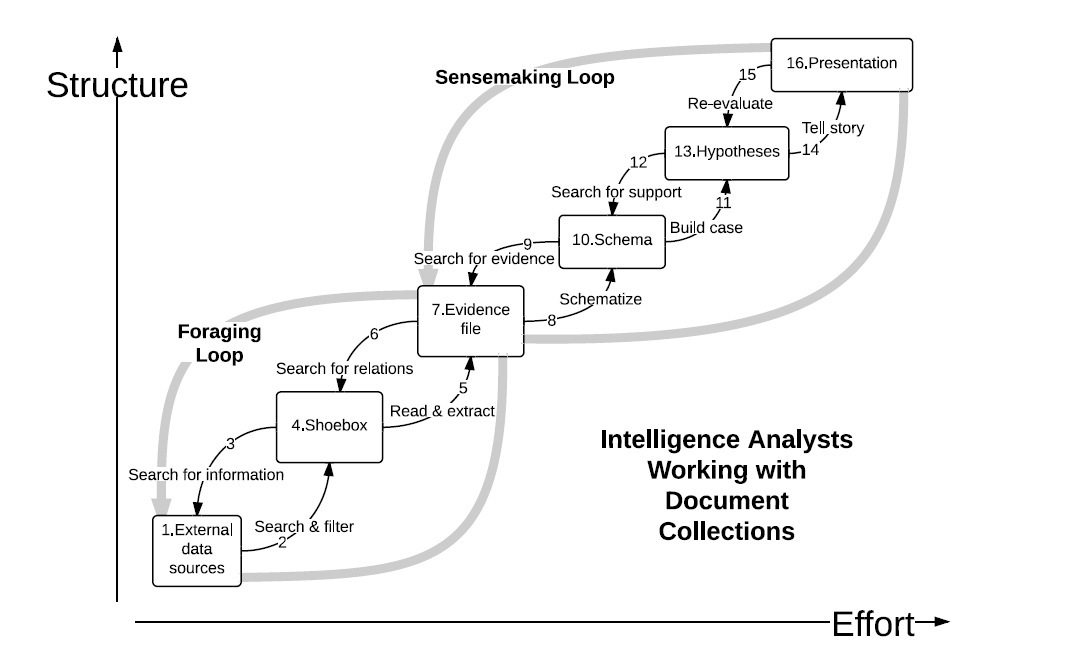
\includegraphics[width=0.9\columnwidth]{images/sensemaking.png}
\caption{Pirolli and Card's sensemaking process for intelligence analysis}
\label{fig:figure2}
\end{figure}


\section{Characterizing web archive research} % (fold)
\label{sec:characterizing_web_archive_research}

% section characterizing_web_archive_research (end)


When discussing web archive research a distinction must be made between studying the web archive itself and using the web archive to study phenomena. Schneider and Foot in \cite{schneider2004web} advocate the archive itself as an object of study that can help gain new insights. Br\"ugger in \cite{brugger2012historical} proposes the study of history based on the evolution of the linking structure of the web archive. He also proposes a study of a nation's web sphere, a large linked set of URLs, over time in order to understand the development of the nation and it's web space. Studies like this treat the archive itself as the cause for the study. On the other hand, researchers are also interested in studying how certain phenomenon evolve or have been discussed on the web. In this case the archive is used to find relevant material for the study rather than being the object of the study.

There is interest from a variety of fields including computer science, digital humanities and the more traditional humanities like history, literature and sociology to study phenomena from our recent past using web archives. The main difference between digital humanities and the humanities though is the former's use of computational methods to study digitized documents. However the web and the archive are not digitized content; they are born digital and reborn digital respectively. Richard Rogers in~\cite{rogers2013digital} advocates the use of digital methods to study the web. Digital methods are a set of practices designed specifically to analyse the web and in turn these can also be applied to web archives. In \cite{huurdeman2013sprint}, Huurdeman et. al. show how digital methods can be applied to the Dutch news archive for analysis. As a result of their work they developed a suite of tools that has been incorporate in the WebArtist system at the University of Amsterdam.

A key point to note is that Rogers also advocates the use of digital methods so that scholars can work at a larger scale which allows them overcome some of the flaws of the web archive as alluded to earlier.

Humanities scholars like historians and sociologists however do not tend to use such computational methods.They spend a lot of their effort in carefully constructing a body of evidence for their hypothesis and then manually analyze this corpus for interesting insights. All humanities and social science scholars share a set of activities when conducting research which are: searching for information, gathering and organizing it, skimming and re-reading it in order to gain new knowledge and assess its importance, note-taking, translating, gathering materials for writing, and constructing a final product \cite{palmer2008scholarship}. This implies that scholars partake in the process of sensemaking and can be accommodated in Br\"ugger's framework for web archive research.

There are also two distinct types of research being carried out with web archive. The first is large scale link analysis. Studies from this domain try to gather insights from the archive by studying how links between pages/ websites/ domains change over time. Links are not readily extractable from web archives though so they need some amount of technical expertise to gather the data. Hence link based studies have generally been carried out by researchers from a more technical background. Internet research institutes and web mining groups in particular are interested in large scale web data and have been responsible from the majority of studies using link analysis. For instance~\cite{hale2014mapping} is one of the latest studies based on web archive link analysis from the Oxford Internet Research Institute. In that paper, they draw conclusions from the UK web space by studying the link relationships between domains over a 14 year time period from 1996 to 2010. The outcomes of this study include the growth of domains in terms of URLs over time and also the relationship between domains based on the link density between them. They do not however go into the content of each URL. Many studies involving web archives have focused on the link structure. Foot et. al. ~\cite{foot2003analyzing} studied the linking practices between electoral candidates during the 2002 elections. In ~\cite{payne2008longitudinal} the link structure between university pages is studied to draw correlations between research productivity and in-links. Toyoda et. al. ~\cite{toyoda2003extracting} go as far as using links between URLs in the Japanese web archive to analyze the evolution of communities on the web. 


%A considerable section of this paper also describes how the data was acquired and the methods used to select, prune and visualise the data needed for the study. 


%To help less technical researchers like humanities scholars get easier access to this kind of data, WebArtist has developed a host of tools for web archive information extraction which have user friendly interfaces.

The second type of research being carried using web archives is the analysis of the content on a given page or set of pages. Here the emphasis is on the page at each URL and not the just the links between pages. Researchers observe a set of web pages to find evidence for their hypothesis rather than writing computer programs to extract evidence. 

\paragraph{A closer look} % (fold)
\label{par:a_closer_look}
% paragraph a_closer_look (end)
Sophie Gebiel, a historian from the Centre d'information et d'{\'e}tudes sur les migrations internationales, studied the history of North African immigration memory in France by using a corpus of web pages collected from the French web archive ~\cite{gebeil2014memoires}. One of the crucial aspects of her work was the definition of a corpus of study. In large scale studies, the criteria for selecting a corpus are usually rudimentary; like all web pages in a domain\/subdomain or all web pages in English. Sophie decided to approach her analysis from both a quantitative and qualitative perspective. Due to the nature of her study, the constraints for selecting a corpus were much stricter. Sophie's work though did not focus on an entire domain but instead on a representative sample, which was selected based on her definition of a relevant corpus, of the whole web archive. Her corpus of study was 70 websites whereas in \cite{hale2014mapping} the corpus was over a few million. The objective of her qualitative study was to understand how memories of North African immigration are portrayed on these websites whereas the quantitative study provided more of a supporting role by providing evidence in the form of network graphs. Qualitative studies such as Sophie's cannot be easily carried out on large corpora which makes the process of selecting a sample very important for her qualitative research. 

Another interesting study performed on the content of web archives rather than the link structure was the analysis of google's home page evolution. Rogers in \cite{rogers2013digital} shows that just by studying the home page of google over a 10 year span we can see the decline of the web directory and the rise of web search. They use a time lapse video to show the change in position of the link to the directory from its most prominent position in the early 2000s to its complete disappearance in 2008.

In the rest of this chapter we pay more attention to the second type of research which is content based research. The next section delves into how researchers, who do not have the expertise to write programs to work with web archives, access web archives to construct corpora and analyze these corpora.


\section{Accessing and analyzing web archives} % (fold)
\label{sec:problems_faced_by_humanities_researchers}

% section problems_faced_by_humanities_researchers (end)

The most popular way for non-technical users to access web archives at the moment is through the wayback machine interface~\cite{wayback}. A user can enter the URL she is interested in to get a list of versions for that URL over time. Selecting one of the versions leads to the HTML file of the version, which is rendered by the browser for the user. The user can also click on the links of the page to be taken to archived versions of anchor URLs if available. The wayback machine allows the user to surf the past web. In the past, with the advent of search engines, surfing became less commonplace and users searched for particular pages instead. 

To search the web archive we need an index. Indexing that amount of data has many challenges to overcome. To avoid the complexity of indexing the world's web archive the IIPC (International Internet Preservation Consortium) indexes small event centric subsets of the web archive instead, like the Socchi Winter Olympics archive \cite{socchi}. Governments across the world have tasked the national libraries with preserving their nation's web and these institutions are working on creating an index for their nation's web archive. For instance, the British Library is responsible for archiving web pages from the \texttt{.co.uk} domain space and for making this archive available to the public. With the help of donations from the Internet Archive, some nations now possess web archives spanning from the early 90s to 2013. There have been successful attempts at indexing web archives like the Portugese web archive \cite{pta} and the Dutch web archive \cite{nla}. They also provide users with keyword search interfaces to access the data. The British Library also provides a search interface to its web archive. Even though this is a big improvement over the wayback machine in terms of access, more fundamental issues exist when accessing and analysing web archives.



%Both types of research can be either qualitative or quantitative. Computer scientists and internet researchers are more adept at working with large data sets due to their technical expertise whereas Humanities scholars are more adept at working with smaller datasets. According to Schneider, Foot and Wouters, the web archive seems to promise novel ways of combining qualitative and quantitative research. 


% understanding how users work in general: sensemaking






% digital methods

%Mining of trends and patterns, studying the past: evolution of a particular page, website, websphere

% Internet research institutes study large scale quantitative data whereas humanities researchers focus on smaller subsets of data


% predominant large scale analysis has been done on links

% small studies focus on content/interface elements

% prominent studies conducted on web archives : case studies from Aarhus and some related work

% interesting insights gained from these studies show the importance of web archive research

% Doughtery's attempts to highlight researchers problems: legal, access and preservation issues

% section types_of_web_archive_research (end)

\section{Understanding researcher access requirements}% (fold)
\label{sec:understanding_researcher_requirements}

In general, research with web archives consists of 4 steps as mentioned before. However these steps are still quite general and the requirements of the researcher can vary greatly depending on the type of study. In the subsequent sections we focus predominantly on humanities scholars and their needs when using web archives. The objective of studying researcher methodology is twofold; first is to understand the overall requirements of a web archive system geared towards humanities research and in turn, secondly to identify open research problems for the computer science community. To better understand humanities web archive methodology, we conducted a series of discussions and interviews with humanities researchers, who have varying degrees of experience of working with web archives.

\subsection{Setup} % (fold)
\label{sub:setup}

The study was conducted with 20 researchers in total. The researchers can be divided into 3 groups based on their experience. The first is the group of scholars that gathered at Aarhus University, Denamrk for a summer school in June 2014. This group represents a set of scholars who have worked quite extensively with web archives. The second group of scholars are the bursary holders from the British Library's web archiving project, BUDDAH (Big UK Domain Data for the Arts and Humanities) \cite{buddah}. These are a group of researchers who are only recently starting to work more closely with web archives. The third group of researchers is the budding Digital Humanities group at the University of Göttingen, Germany. Here the experience with web archive based research is for all intents and purposes, negligable. 

The format of the discussions was varied in each case due to the setting and venue. Most were open ended discussions that centered on the methodolgy used for research and in particular the problems faced when doing so. One of the methods considered for the interview process was the ACTA technique \cite{militello1998applied}. This method is a streamlined version of the Cognitive Task Analysis methods for identifying cognitive skills, or mental demands, needed to perform a task proficiently. However for this technique to be applied, all participants in the interview process should share a similar level of experience. The experience of the interviewed researchers with web archives though varies from over 10 years for Niels Br\"ugger to no experience for Gerhard Lauer. But each individual brings a certain perspective to research in web archives which should be considered when trying to understand their needs.
This approach of bringing humanities scholars in contact with developers and computer scientists to improve web archive systems has been advocated strongly in technical reports like \cite{dougherty2010researcher}. 

In the subsequent sections we discuss the insights gained based on data gathered during discussions regarding the participants methodology and problems faced.

\subsection{Insights on research methodology} % (fold)
\label{sub:data}

Over the course of the summer school in Aarhus University, I indulged in several interviews and group discussions with the researchers. We also participated in the presentations made regarding their wrok. There were presentations regarding both qualitative and quantitative research on web archives. 

Researchers more used to a qualitative approach doubted the consistency and quality of the data used in large scale quantitative analysis whereas some researchers doubted the validity of results produced on small albeit high quality samples of the archive. What was immediately clear to us and everyone present though was the potential of web archives to combine both types of research if certain points could be addressed. This was alluded to by Schneider and Foot as well in \cite{schneider200911}. An excerpt from their report that sheds more light on this is shown below:

\paragraph{} % (fold)
\label{par:}

% paragraph  (end)
'Web archiving does seem to promise novel ways to combine quantitative and qualitative research in one design. First of all, the fact that the datasets can be huge will enable qualitative researchers to check whether a particular phenomenon or pattern they have found in one particular case also seems to be relevant if one looks at a large number of case studies. This could technologically be supported by “pattern matching” software tools (either in the form of Perl or Python scripts, or in NVivo or Atlas.ti type of tools). Second, qualitative data pertaining to a particular case study can be represented as a node in a network, thereby possibly contributing to a bet ter feel for the ‘place’ of one’s case. Third, Web archiving methods enable researchers to collect a variety of quantitative data as harvested metadata. This minimizes the effort on the side of the researcher while still enabling her to couple her own data (whether quantitative or qualitative) to these meta-data. And lastly, quantitative research designs may be enhanced by exploration of concrete instances (e.g., Web pages) of phenomena about which one has quantitative data.'

\paragraph{} % (fold)
\label{par:}
Apart from the suggestions made by Schneider and Foot, we believe for humanities scholars more used to working qualitatively with text documents they need to better understand the limitations of a web archive. For humanities scholars beginning to work with web archives there are 2 main concerns: the absence of all versions of web pages and the timestamp for each is only the crawl date and not the actual publication date. Since their collections are often small samples, the consistency and quality of these samples must be very high. These inconsistencies can be glossed over however when taking a large enough sample. This is probably why we have seen more large scale link based analysis as the predominant mode of study for web archives. In order to encourage more humanities researchers to use existing web archive data it is imperative for them to understand the limitations of the crawlers and also define a set of error boundaries when defining their small corpus. By gaining a better insight into some of the technical challenges behind creating an archive, in my opinion, humanities scholars can define select a reasonable corpus and motivate its usage despite its shortcomings. 

What we found most surprising though was the corpus creation procedure for many of the studies. The large scale studies were based on broad domain based selection whereas the small scale qualitative studies were based on human curated list of URLs. This is mostly due to the nature of the primary access point for web archives, the wayback machine. The wayback machine acts as a look up service which given a URL as input will show the list of versions available and render the content of each version when requested. This sort of access doesn't allow for any kind of search or exploration. To build a corpus of relevant web pages, scholars should not have to manually build catalogs of URLs. A search feature is paramount to helping them find more relevant pages and sites for their corpus. To enable search though, the archive needs to be indexed. This is not a trivial task given the sheer size of just 10-15 years worth of web archive data. To date there have been only a handful of large scale web archive indexes like the Portugese Web Archive and British Web Archive. The IIPC chooses not to index the whole web archive but instead create indexes for pages related to particular topics or events. The participants in the summer school had not been exposed to a full text web archive search system during their work and hence relied on the wayback machine.

Another interesting discussion that came up was centered around the first of Schneider and Foot's suggestions to combine both forms of research. The question raised by Leigh Graham was: how can I check if my hypothesis is valid on all discussions about my subject not just the small sample I have worked with? Pattern checking is one possibility while the other is the actual scaling up of the theory behind the hypothesis. This is closely related to Mathew Webber's work on 'big theory'. 

%imp
There is a need to translate these theories to a web scale, where the primitives need to be redefined as simple formulas that can be applied to large aggregates of the whole dataset. In essence if we can define theory from the social sciences and humanities as precise mathematical formulas then we can approximate the variables used accordingly and try to evaluate the theory on a much larger scale.

For scholars like Frederico Nanni, a historian at the University of Bologna, there is a great deal of interest in studying web archives using a combined qualitative and quantitative approach. He wanted to use LDA (Latent Dirichlet Allocation) to generate topic models in order to study the evolution of topics in Italian university websites. However without programming knowledge, both extracting the data and building a topic model is very difficult today. This hurdle of technical expertise discourages a lot of humanities scholars from utilizing the full scale of web corpora. There is a need to build systems that incorporate algorithms like LDA based topic modeling in a user friendly manner.  

%imp
For scholars who are not aware of the strengths and weaknesses of the algorithms it can seem like using these methods creates an inherent bias. But if researchers can gain more transparency to the working of mining algorithms then they can use it more effectively and also describe it more accurately. A simple way of adding transparency is to allow users to tweak the parameters for algorithms and see how the output can is affected.For example, in any form of clustering we need to set the number of clusters k. Why not let the researchers vary these values and observe the effects. Easy to use tools with transparent algorithms is key to helping humanities scholars.


\subsection{Insights on corpus creation and web archive search} % (fold)
\label{sub:data_gathering_ii}

After getting an overview of some of the more general problems faced by researchers when working with web archives, we decided to focus on the following subset of researchers: humanities researchers using the web archive as a source for a predominantly qualitative study. The BUDDAH project at the British Library, London, is an effort to encourage humanities scholars to use web archives. To encourage scholars to work with archives an adequate system needs to be in place first. Another major goal of the BUDDAH project is the development of a system suitable for scholarly access to web archives by working in tandem with scholars. The British Library possess over 15 years of the UK web (.co.uk) gathered by their own crawls and donations from the Internet Archive. As part of the BUDDAH project, a bursary scheme was announced at the beginning of the project to select candidates to work with web archives. Candidates were asked to send in applications describing the topic they want to study using web archives and also the methodology they would employ if selected. A total of 11 applicants were chosen and given access to the British Library's web archive search system. At the time of interviews only a random 12\% sample of the entire dataset was indexed and made available to the users. The index for the whole dataset was close to completion at the time and the intention was to swap the indices and retain the same interface.

The very first step for any scholarly work is the formation of a corpus. As seen from the sensemaking model by Pirolli and Card, the first stage of corpus creation is exploration of the data. To help scholars explore this large UK web archive dataset they indexed it so as to make it accessible to keyword search. Keyword search is a better choice to explore the archive if you are unaware of the URLs you actually want to use. The search functionality provided to all scholars is keyword based faceted search. The facets are based on the domains and subdomains of the resulting documents as well as the crawl date. There is a form that users can use to specify advanced search functionality as well like: phrase search, proximity search, etc. A negative keyword filter was also made available to remove spam results. 

At the time of our meeting with the bursary holders and members of the BUDDAH project, scholars had just begun working with the search system and trying various keywords to find some relevant documents. We had a group discussion with both the developers of the system and the bursary holders to try and understand the challenges they were facing. We also had the chance to study the applications of the scholars. These applications proved to be an invaluable source for understanding the intent of the scholar when they use the search system to explore the archive.

Overall the scholars were happy with the search features provided. They did find it difficult to find the right set of keywords to express their intent though. Upon closer analysis of the applications though we found that users wanted all documents related to a certain topic. The topics can have multiple facets which are not evident to the user straight away from the search results. For example when one of the users was searching he found a large number of results from amazon which were irrelevant to his study. To overcome this he had to add the word 'amazon' to the negative keyword list and repeat his search only to find more 'spam'. 

We found that almost all users were using advanced queries to narrow down their results to a number small enough that they could go through manually. One major feature that was requested by the scholars was an ability to create corpora from within the system. Some users resorted to using a spreadsheet to keep track of the web pages selected along with thew keywords used. As with any form of scholarship the documentation of corpora formation is key to replicating the study. The engineers at the British Library at the time had decided to add a simple corpus creation feature where users could add relevant results from the search page to a user defined bucket. Based on this feature, the scholars also requested a possibility to export the results in a suitable format for their analysis of this dataset. If the system in itself is only for search and not for analysis then exporting of corpora becomes the link that joins stage 1 and 2 of Br\"ugger's framework. 

A web archive search system for scholars should support at the very least the following tasks:

\begin{itemize}
	\item Exploration: search using keywords with advanced querying like phrase match and proximity at the very least. There exists a rich body of work on content analysis and data mining that can help users explore corpora more intelligently.
	%cite zeon's thesis
	\item Selection and documentation: The system should also document in detail the actions of the user when selecting search results for his corpus similar to the search history. Citing is a key concern for scholars. To cite web objects they need, not only keywords used to locate them but also the crawl meta data from where the object came from.
	\item Export: exporting a corpus with its documentation in popular formats like CSV and JSON so that further analysis can be done with tools that researchers are already comfortable with. 
\end{itemize}

 \textit{A consequence of detailed user tracking should be the use of relevance feedback techniques to improve the search process. To the best of our knowledge relevance feedback in web archive search has yet to be studied.}

An example of web archive search system developed for scholars is the WebArtist initiative~\cite{huurdeman2013sprint}which combines search with better data visualization and rudimentary aggregates. It also allows users to export their results in CSV.

\paragraph{} % (fold)
\label{par:}
% paragraph  (end)
%imp
The rest of the issues discussed that day were centered around the search interface and results. Overall the users were satisfied with the result presentation in the 10 blue links paradigm. The search results themselves are hard to comprehend with large number of versions for each page. The ranking of search results in their system is time ordered so as to not get clusters of versions of the same URL in the result list. This method is rudimentary at best and really points to the need for better search result ranking and visualization paradigms. Costa et al \cite{costa2010understanding} have already shown that standard IR ranking models do not produce satisfactory results for users of web archives. There is a need for models that are time and version aware. An interesting point to note is also the scholars need to avoid bias. Time ordering is easy to understand and explain when describing the corpus creation process using search. However with ranking algorithms, the scholars feel the system is introducing a certain amount of bias. Scholars need to better understand the objective of each ranking algorithm so that they can use it when the need arises and explain it in their work. This is once again a case of algorithms being made transparent and known to the user when they are being employed. 

\paragraph{Bursary applications} % (fold)
\label{par:bursary_applications}

% paragraph bursary_applications (end)
We shift our focus to the bursary applications of the scholars selected to work with the archive. Each bursary application consists of the following fields: General subject area, Title of the study, Description of the study (500 words), Proposed methodology (200 words) and the benefits of the research. To maintain the privacy of the bursary holders I will not be delving into their areas of research in detail. Instead I will focus on their methodology for corpus creation and analysis. Since the dataset is the UK web archive from 1996 to 2013 the scholars chose topics which are relevant to the UK. The scholars come from a variety of disciplines ranging from the medical domain to history. First I classify the studies based on the scale of study suggested in the proposal. Out of 11 participants all chose small scale studies where they would construct the corpus of study manually using a combination of keywords and filters for search. 2 scholars also consider large scale studies to determine trends. 2 out of 11 scholars also restrict themselves to only a particular subdomain within the entire UK domain space. 1 participant wants to compare her results against results from the live web. 5 of the scholars explicitly propose to use popular or leading URLs from their field of study as starting points for corpus creation. This approach can be flawed due to the fact that web pages do change addresses over time. All participants however used the keyword search feature to start exploring the dataset. 2 scholars want to build their corpus purely based on keywords and no restrictions in terms of types of websites. Some scholars are more interested in the social aspect of the web like blogs, forums and discussions; while others in the more formal authoritative websites like an organization's main website. 1 scholar expressed his interest in studying an image archive from the UK web archive, which we believe can be an interesting problem to solve. \textit{It is interesting to note that in most cases the web page is considered the first class citizen in search but users could be interested in rather specific elements on each page. A closer look could be taken at the indexing granularity to cater to these needs.}

In terms of analysis, most users were happy to visualize the link structure in the corpus they were going to create. 2 participants made the link structure of their corpus their main focus. 7 of the 11 scholars explicitly state an interest in studying their subject over time using terms like evolution and understanding the past in the description of the study. While most participants were interested in the content of the web pages in the archive, 2 scholars were particularly interested in the HTML structure of the pages they collect. The type of analysis they will conduct on the final curated corpus varied from scholar to scholar. Only 3 scholars wanted to conduct quantitative studies. 

%imp
 \textit{During discussions with the scholars, we found that generating keywords to find relevant documents for their topic was a tedious task.} The web pages they were looking for were not annotated with any kind of topical taxonomy. The more metadata there is regarding the type of the web page and the topics covered, the easier it will be for researchers to search for relevant material faster. Another major concern for researchers was how to get an overview of the result sets when even after filtering the result set was over a few thousand documents. The current time ordered ranking is neither helpful in terms of finding the most relevant documents nor getting an overview of the result set.

% even for the ones who are aware of the URLs they want to study there is no´guarantee that the same URL has stayed constant over the years.
In the next section, we make a case for better methods to help search and exploration in web archives and use this as motivation to develop a novel retrieval model for archive search.
% subsection data_gathering_ii (end)

% subsection subsection_name (end)
%josh, megan, leigh, sophie, anat, frederico, 11, frank fischer, gerhard lauer

% subsection setup (end)
% trying to understand how researchers at the BL are conducting research

% Setup: 13 year archive, keyword search system, bursary scheme

% Each researcher describes his work with a short proposal whcih can be seen as the detailed user intent.

% present 4 intents

% discuss the initial progress of these researchers and the problems faced by them: choosing keywords, missing
%versions, ranking by time, have to go through every result, what do we do when there are a large number of relevant results


% My understanding of what researchers want: scale up problem, we want everything, confidence measures, algorithms that are user friendly, forming a subcorpus, exporting subcorpus, citing, documentation

% section understanding_researcher_requirements (end)

\section{Intelligent access to web archives} % (fold)
\label{sec:intelligent_access_to_web_archives}

\paragraph{Recap} % (fold)
\label{par:recap}
To form a corpus of study from a web archive scholars need effective ways to access the data in the archive. Until recently the most commonly used form of access was the wayback machine service. This kind of lookup service is useful when you only want to study a limited set of URLs. To allow researchers to search the corpus with keywords rather than URLs, national libraries and the IIPC have taken to indexing either their whole collection or parts of it. Search is already a major improvement compared to the wayback machine for access. 

For an access method to be considered intelligent it should have features that make it easier for the user to quickly access the data they are interested in. Search in itself is a generic access method but it can be considered to be an intelligent method of access for web archives with the addition of domain and time based filtering. However even with these features researchers we have observed scholars having to do a lot of manual filtering to find relevant documents.

Search should not only find all documents containing the keywords but also rank more relevant documents closer to the top. By ranking the most relevant documents towards the top we save the user time and effort.Web archives though pose their own set of challenges for search result ranking due to the temporal version-ed nature of the documents in the collection. Costa et al. have already shown that traditional IR retrieval models are not very good when used for web archives. We also observe that with the British Library's decision to rank results in descending order of timestamp instead of using the baseline retrieval models provided by Solr. Traditional retrieval models are time averse so it is extremely likely that the top k search results for a query could be different versions of the same document across time.

Let us look more closely at a select set of the bursary applications to understand the information seeking nature of certain scholars. Once again, we will refrain from going into the actual research topic but instead try to abstract the scholars intention alone.

%imp
\paragraph{Case 1:} % (fold)
\label{par:paragraph_name}
The scholar wants to study the evolution of the reception by the online community towards a certain topic, say X. This topic can be expressed by keywords. In the application, the scholar mentions entities relevant to the topic as well that could be used as keywords. The information intent of the author can be interpreted as: I want to get documents from different time periods about X. These documents should provide an opinion of a person or a group about topic X.

\paragraph{Case 2:} % (fold)
\label{par:paragraph_name}
The scholar wants to study the blogs from a community C chronologically. The scholar more specifically states that she wants blogs that mention a particular aspect A. Once she has the blogs she would like to find patterns in them. The intent can be expressed using keywords that describe the community. Filters can be used to narrow down results to the blogosphere as well. The complete user intent however can be interpreted as: I want to get all relevant blogs from C that mention A from different time intervals that possess documents about community C.

\paragraph{Case 3:} % (fold)
\label{par:paragraph_name}
The scholar wants to study the history of politician P. The scholar wants to know the interesting facts about the life of P from various aspects. The intent is represent as keywords which in this case is the name of politician P. The user intent when studied more closely can be interpreted as: I want to get all documents that cover diverse aspects of P's life.

From the cases mentioned above, we can see that inherently scholars want results which are diverse. Scholarly search in web archives can be considered as a high recall high precision task. Scholars want not only relevant documents but documents which are from important and diverse time intervals and cover a broad range of aspects. By diversify we also provide the user with a brief overview of the result set. We believe that one of the ways to make the current search methods for web archives more intelligent is to to add diversity; diversity not just over time but also over aspects. 

In the next chapter we motivate and develop a retrieval model for scholars whose search intent is to study the evolution or history of a topic.



%access methods are needed to form subcorpora or explore the corpus for relevant documents to test your hypothesis

% current access methods: keyword search, filtering by domain, wayback machine

% intelligent access: getting exactly what you want and getting an overview

% researchers shouldn't have to comb through the data to find important time periods and content

% this can be mined and presented to the user while he tries to access the data so that he can make more informed to decisions on which documents he needs to study. save time and effort. cut out the rudimentary parts of research by allowing machines to filter automatically and present data driven overviews

% current search is very limited: ranking? query suggestions? query expenasions? relevance feedback?

% mining algorithms can be used to generate corpus overviews and present users with an entry point

% documentation of the user's progress is essential for reproducing the study


% section intelligent_access_to_web_archives (end)

% chapter researcher_engagement_with_web_archives (end)